\subsection{Running \thename{}}
\label{sec:appendix:make}

Building \thename{} is a simple matter of using the GNU Make build tool. In the
root folder containing the file \code{Makefile} simply run the command
\code{make} to build and run the machine with the hardcoded test program.

Tests are likewise run via make using the command \code{make test}. Valgrind
analysis and gprof profiling is performed with \code{make analyze} and
\code{make gprof}, respectively.

\subsection{\thename{} Specification}
\label{sec:appendix:spec}
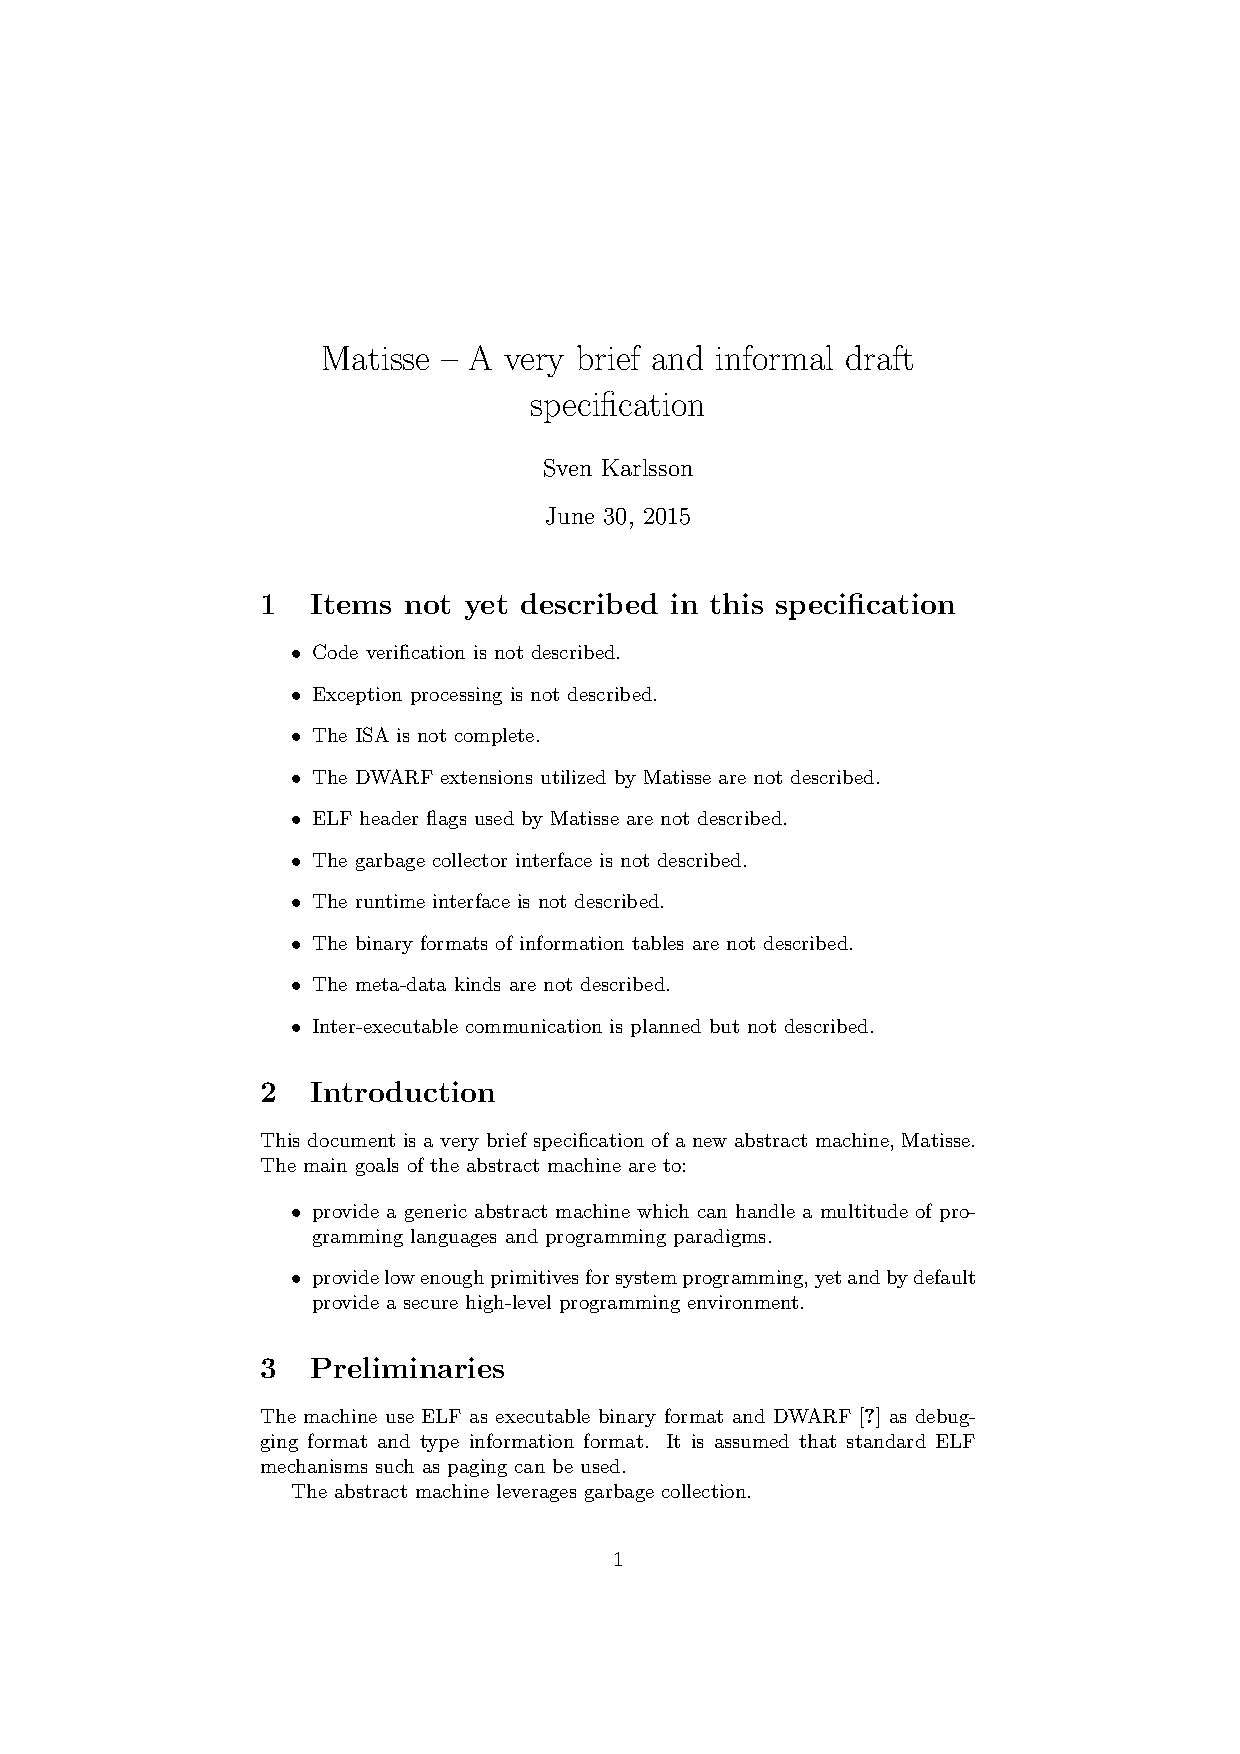
\includepdf[pages=-]{lib/spec.pdf}

\subsection{Project Inception Phase Artifact}
\label{appendix:inception-artifact}

\includepdf[pages=-]{lib/Inception.pdf}

\subsection{Risk Assesment Analysis}
\label{appendix:risk-assessment}
%TODO

\subsection{Benchmark Runner}
\label{appendix:benchmark}
\begin{lstlisting}[language=bash]
#!/usr/bin/bash
# benchmark runner
# based off:
# https://gist.github.com/peterjmit/3864743

repeat=1
step=1
range_from=0
range_to=30
output_file="benchmark.csv"
command=""

run_tests() {
    echo "benchmarking: ${command} ${range_from}..${range_to} (step ${step})"

    # truncate output file
    if [ -f ${output_file} ]
    then
        > ${output_file}
    fi

    # print column names
    echo "round,n,time,user,kernel" >> ${output_file}

    # repeat
    for (( j = 0; j < ${repeat}; j++ ))
    do
        # for each in range
        for (( i = ${range_from}; i < ${range_to}; i += ${step} ))
        do
            # percentage completion
            p=$(( ($i + 1) * 100 / $range_to ))
            # indicator of progress
            l=$(seq -s "#" $(($p / 2)) | sed 's/[0-9]//g')

            # time command
            /usr/local/bin/time -f "${j},${i},%e,%U,%S" -o ${output_file} -a ${command} ${i} > /dev/null

            # clear the HDD cache (i hope?)
            sync && echo 3 > /proc/sys/vm/drop_caches

            printf "%s/%s: %-48s %3s%%\r" "$(($j + 1))" "$repeat" "$l" "$p"
        done
    done

    echo -ne '\n'
}

# Option parsing
while getopts s:f:t:n:c:o: OPT
do
    case "$OPT" in
        s)
            step=$OPTARG
            ;;
        f)
            range_from=$OPTARG
            ;;
        t)
            range_to=$OPTARG
            ;;
        n)
            repeat=$OPTARG
            ;;
        o)
            output_file=$OPTARG
            ;;
        c)
            command=$OPTARG
            ;;
        \?)
            echo 'error: failed to parse args'
            exit 1
            ;;
    esac
done

shift `expr $OPTIND - 1`

if [[ $command == "" ]]
then
    echo 'error: no command to run'
    exit 1
fi

run_tests
\end{lstlisting}

%%% Local Variables:
%%% mode: latex
%%% TeX-master: "../report"
%%% End:
